\documentclass[10pt]{article}
\usepackage[colorlinks=true,linkcolor=black,urlcolor=black,citecolor=black]%
{hyperref}
\usepackage{proof}
\usepackage{amsmath}
\usepackage{cite}
\usepackage{graphicx}
\usepackage{stmaryrd}

\title{Artisanal type theory}
\author{Carlo Angiuli}
\date{April 1, 2015}

\begin{document}
\maketitle

\section{A brief history of some things}

Food was invented by Mesopotamians some 5,000 years ago, and has been eaten ever
since. 
%
Logic was invented in the Mediterranean by ancient Greeks, including Aristotle
and a mortal man \cite{Aristotle40} named Socrates. It lives on as an important
course in pre-law curricula across the United States. 

Modern times require more modern logics. Computer programming is closely tied to
\emph{intuitionistic} logic, in which proofs of a proposition correspond
directly to algorithms. Intuitionistic logic, often in the form of type theory,
is taught to several American computer scientists annually.

Until the past several centuries, food and logic were primarily manufactured by
artisans, who trained apprentices in the arts of, respectively, proofing and
proving.
%
The Industrial Revolution gave rise to machines able to produce food and
textiles much faster than artisans ever could.
%
The digital revolution, likewise, has turned `computer' from a human job into a
cheap, ubiquitous machine capable of multiple calculations per second.

Despite the overwhelming success of mass-produced food, some consumers want to
revisit food's roots as a product sustainably and ethically crafted by local
artisans using traditional techniques. The result, known as \emph{artisanal
food}, has taken off in popularity in the past few years \cite{NYT09,Cope14}.

\section{Algorithms with the human touch}

So too should computer scientists return to the roots of computation---slow,
error-prone calculations performed by humans. After all, despite the close
relationship between computer programs and type theory \cite{MartinLof85}, or
indeed, between computer programs and algorithms, there is no need to involve
computers in deeply human tasks like sorting lists, routing packets, or decoding
MPEG-4 video streams.

We advocate a more personal approach to computation, called \emph{artisanal type
theory}. Artisanal type theory has the same rules as ordinary type theory,
except that all terms and typing derivations must be handwritten. Closed,
well-typed terms evaluate to values of the same type, accompanied by a
certificate of authenticity that a human performed that evaluation.

Since each term was lovingly handcrafted and normalized, these
artisanally-performed beta-reductions provide a more \emph{meaningful}
explanation of type theory than traditional computer-based interpreters.
Using artisanal type theory demonstrates a firm commitment to
\emph{locally-}grown, sound, and complete reasoning systems.

\section{Examples}

\paragraph{Shallow learning.}
We can implement artificial intelligence using human intelligence. Given the
training data that \texttt{false} is desired but \texttt{true} is not, one can
manually build a classifier for booleans. Such a classifier can then be run on a
boolean to determine whether or not it is in the desired set. In the example
below, we run the classifier on \texttt{false}.

\vspace{1em}\noindent
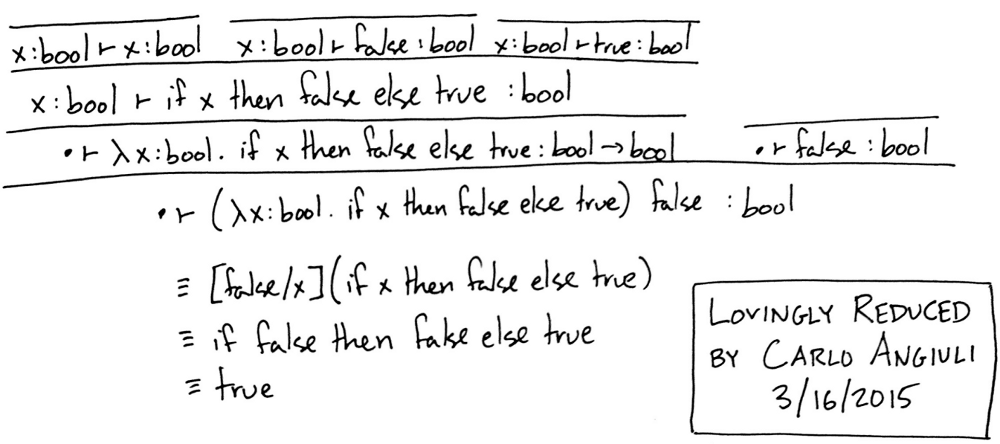
\includegraphics[width=\textwidth]{isfalse.png}

\paragraph{Fairly quick sorting.}
Artisanal computation has some advantages over computer programming---namely,
humans can perform some computations without needing a precise algorithm.
In this example, we sort a list of integers without the need to specify a
particular sorting algorithm.

\vspace{1em}\noindent
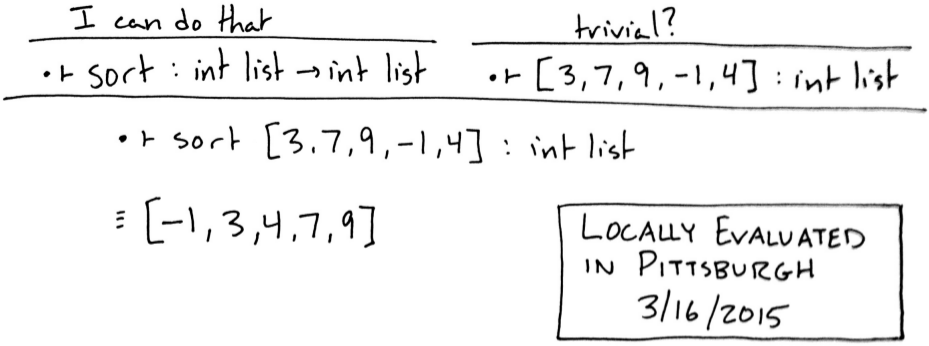
\includegraphics[width=\textwidth]{sort.png}

\paragraph{Small-batch jobs.}
We can also write scripts which artisanally perform repetitive computing tasks
such as renaming a large number of files, accessing sequential URLs, etc. Doing
so requires adding primitives for I/O, file system access, and so forth. As
discussed above, it is unnecessary to actually implement these primitives,
because the human runtime already supports these tasks via a computer's
traditional user interface.
%
Furthermore, unlike in traditional scripting languages, it is easy to extend
this with physical-world primitives such as \texttt{eatLunch},
\texttt{writeHandwrittenThankYouNote}, and \texttt{sleep}.

\section{Conclusion}

We hope artisanal type theory will appeal to computer scientists and
mathematicians who appreciate algorithms but believe computers themselves are
quite inconvenient at times. Unlike ordinary type theory, it directly expresses
computations as if people, but not computers, matter. Therefore, we are hopeful
that artisanal type theory will be a useful foundation for the field of
\emph{human science}.

\bibliography{artisanal}{}
\bibliographystyle{acm}

\end{document}
